% (find-LATEX "2021-1-C3-matriz-jacobiana.tex")
% (defun c () (interactive) (find-LATEXsh "lualatex -record 2021-1-C3-matriz-jacobiana.tex" :end))
% (defun C () (interactive) (find-LATEXsh "lualatex 2021-1-C3-matriz-jacobiana.tex" "Success!!!"))
% (defun D () (interactive) (find-pdf-page      "~/LATEX/2021-1-C3-matriz-jacobiana.pdf"))
% (defun d () (interactive) (find-pdftools-page "~/LATEX/2021-1-C3-matriz-jacobiana.pdf"))
% (defun e () (interactive) (find-LATEX "2021-1-C3-matriz-jacobiana.tex"))
% (defun o () (interactive) (find-LATEX "2021-1-C3-matriz-jacobiana.tex"))
% (defun u () (interactive) (find-latex-upload-links "2021-1-C3-matriz-jacobiana"))
% (defun v () (interactive) (find-2a '(e) '(d)))
% (defun d0 () (interactive) (find-ebuffer "2021-1-C3-matriz-jacobiana.pdf"))
% (defun cv () (interactive) (C) (ee-kill-this-buffer) (v) (g))
%          (code-eec-LATEX "2021-1-C3-matriz-jacobiana")
% (find-pdf-page   "~/LATEX/2021-1-C3-matriz-jacobiana.pdf")
% (find-sh0 "cp -v  ~/LATEX/2021-1-C3-matriz-jacobiana.pdf /tmp/")
% (find-sh0 "cp -v  ~/LATEX/2021-1-C3-matriz-jacobiana.pdf /tmp/pen/")
%     (find-xournalpp "/tmp/2021-1-C3-matriz-jacobiana.pdf")
%   file:///home/edrx/LATEX/2021-1-C3-matriz-jacobiana.pdf
%               file:///tmp/2021-1-C3-matriz-jacobiana.pdf
%           file:///tmp/pen/2021-1-C3-matriz-jacobiana.pdf
% http://angg.twu.net/LATEX/2021-1-C3-matriz-jacobiana.pdf
% (find-LATEX "2019.mk")
% (find-CN-aula-links "2021-1-C3-matriz-jacobiana" "3" "c3m211j" "c3j")

% «.video-1»			(to "video-1")
% «.video-2»			(to "video-2")
% «.defs»			(to "defs")
% «.title»			(to "title")
% «.exercicio-1»		(to "exercicio-1")
% «.preparacao-mini-teste»	(to "preparacao-mini-teste")
% «.mt-dica-contas»		(to "mt-dica-contas")
%
% «.djvuize»	(to "djvuize")


% «video-1»  (to ".video-1")
% (c3m211ja       "video-1")
% (find-ssr-links     "c3m211j" "2021-1-C3-matriz-jacobiana" "kMGtZk5er9w")
% (code-eevvideo      "c3m211j" "2021-1-C3-matriz-jacobiana" "kMGtZk5er9w")
% (code-eevlinksvideo "c3m211j" "2021-1-C3-matriz-jacobiana" "kMGtZk5er9w")
% (find-c3m211jvideo "0:00" "5/ago/2011")
%
% «video-2»  (to ".video-2")
% (c3m211ja       "video-2")
% (find-ssr-links     "c3m211j2" "2021-1-C3-matriz-jacobiana-2" "D_YKka3RG9E")
% (code-eevvideo      "c3m211j2" "2021-1-C3-matriz-jacobiana-2" "D_YKka3RG9E")
% (code-eevlinksvideo "c3m211j2" "2021-1-C3-matriz-jacobiana-2" "D_YKka3RG9E")
% (find-c3m211j2video "0:00" "27/ago/2021")


\documentclass[oneside,12pt]{article}
\usepackage[colorlinks,citecolor=DarkRed,urlcolor=DarkRed]{hyperref} % (find-es "tex" "hyperref")
\usepackage{amsmath}
\usepackage{amsfonts}
\usepackage{amssymb}
\usepackage{pict2e}
\usepackage[x11names,svgnames]{xcolor} % (find-es "tex" "xcolor")
\usepackage{colorweb}                  % (find-es "tex" "colorweb")
%\usepackage{tikz}
%
% (find-dn6 "preamble6.lua" "preamble0")
%\usepackage{proof}   % For derivation trees ("%:" lines)
%\input diagxy        % For 2D diagrams ("%D" lines)
%\xyoption{curve}     % For the ".curve=" feature in 2D diagrams
%
\usepackage{edrx21}               % (find-LATEX "edrx21.sty")
\input edrxaccents.tex            % (find-LATEX "edrxaccents.tex")
\input edrx21chars.tex            % (find-LATEX "edrx21chars.tex")
\input edrxheadfoot.tex           % (find-LATEX "edrxheadfoot.tex")
\input edrxgac2.tex               % (find-LATEX "edrxgac2.tex")
%
%\usepackage[backend=biber,
%   style=alphabetic]{biblatex}            % (find-es "tex" "biber")
%\addbibresource{catsem-slides.bib}        % (find-LATEX "catsem-slides.bib")
%
% (find-es "tex" "geometry")
\usepackage[a6paper, landscape,
            top=1.5cm, bottom=.25cm, left=1cm, right=1cm, includefoot
           ]{geometry}
%
\begin{document}

%\catcode`\^^J=10
%\directlua{dofile "dednat6load.lua"}  % (find-LATEX "dednat6load.lua")

% %L dofile "edrxtikz.lua"  -- (find-LATEX "edrxtikz.lua")
% %L dofile "edrxpict.lua"  -- (find-LATEX "edrxpict.lua")
% \pu

% «defs»  (to ".defs")
% (find-LATEX "edrx15.sty" "colors-2019")
%\long\def\ColorRed   #1{{\color{Red1}#1}}
%\long\def\ColorViolet#1{{\color{MagentaVioletLight}#1}}
%\long\def\ColorViolet#1{{\color{Violet!50!black}#1}}
%\long\def\ColorGreen #1{{\color{SpringDarkHard}#1}}
%\long\def\ColorGreen #1{{\color{SpringGreenDark}#1}}
%\long\def\ColorGreen #1{{\color{SpringGreen4}#1}}
%\long\def\ColorGray  #1{{\color{GrayLight}#1}}
%\long\def\ColorGray  #1{{\color{black!30!white}#1}}
%\long\def\ColorBrown #1{{\color{Brown}#1}}
%\long\def\ColorBrown #1{{\color{brown}#1}}
%\long\def\ColorOrange#1{{\color{orange}#1}}
%
%\long\def\ColorShort #1{{\color{SpringGreen4}#1}}
%\long\def\ColorLong  #1{{\color{Red1}#1}}
%
%\def\frown{\ensuremath{{=}{(}}}
%\def\True {\mathbf{V}}
%\def\False{\mathbf{F}}
%\def\D    {\displaystyle}

\def\C{\mathbb{C}}

\def\drafturl{http://angg.twu.net/LATEX/2021-1-C3.pdf}
\def\drafturl{http://angg.twu.net/2021.1-C3.html}
\def\draftfooter{\tiny \href{\drafturl}{\jobname{}} \ColorBrown{\shorttoday{} \hours}}



%  _____ _ _   _                               
% |_   _(_) |_| | ___   _ __   __ _  __ _  ___ 
%   | | | | __| |/ _ \ | '_ \ / _` |/ _` |/ _ \
%   | | | | |_| |  __/ | |_) | (_| | (_| |  __/
%   |_| |_|\__|_|\___| | .__/ \__,_|\__, |\___|
%                      |_|          |___/      
%
% «title»  (to ".title")
% (c3m211jp 1 "title")
% (c3m211ja   "title")


\thispagestyle{empty}

\begin{center}

\vspace*{1.2cm}

{\bf \Large Cálculo 3 - 2021.1}

\bsk

Aula 21: a matriz jacobiana

\bsk

Eduardo Ochs - RCN/PURO/UFF

\url{http://angg.twu.net/2021.1-C3.html}

\end{center}

\newpage

Comece relendo o trecho ao redor da

página 256 no capítulo 7 do Bortolossi...

Hoje nós vamos ver dois jeitos de visualizar

o que a matriz jacobiana quer dizer.

\bsk

Vamos trabalhar em cima de um exemplo só:

a função que leva cada número complexo $z∈\C$

em $z^2∈\C$.

\msk

\ColorRed{Veja os vídeos!}

\msk

Vídeo 1:

{\footnotesize

\url{http://angg.twu.net/eev-videos/2021-1-C3-matriz-jacobiana.mp4}

\url{https://www.youtube.com/watch?v=kMGtZk5er9w}

}

\ssk

Vídeo 2:

{\footnotesize

\url{http://angg.twu.net/eev-videos/2021-1-C3-matriz-jacobiana-2.mp4}

\url{https://www.youtube.com/watch?v=D_YKka3RG9E}

}



\newpage

Porque a jacobiana de $w=z^2$ é desse jeito?

$$\begin{array}{rcl}
  w &=& z^2 \\
  z &=& x+iy \;\;=\;\; (x,y) \;\;=\;\; \psm{x \\ y} \\
  w &=& a+ib \;\;=\;\; (a,b) \;\;=\;\; \psm{a \\ b} \\[5pt]
  \psm{a\\b} &=& w \\
        &=& z^2 \\
        &=& (x+iy)^2 \\
        &=& x^2 + 2ixy + i^2y^2 \\
        &=& x^2 + 2ixy  - y^2 \\
        &=& (x^2 - y^2) + i(2xy)   \\
        &=& (x^2 - y^2, 2xy) \;\;=\;\; \psm{x^2-y^2 \\ 2xy}  \\
      a &=& x^2 - y^2 \\
      b &=& 2xy \\
  \end{array}
$$

\newpage

Porque a jacobiana de $w=z^2$ é desse jeito? (2)

$$\begin{array}{rcl}
  w_z Δz &=& \frac{d \psm{a\\b}}{d \psm{x\\y}} \pmat{Δx\\Δy} \\
         &=& \pmat{a_x & a_y \\ b_x & b_y} \pmat{Δx\\Δy} \\
         &=& \pmat{a_x Δx + a_y Δy \\ b_x Δx + b_y Δy} \\
         &≈& \pmat{Δa \\ Δb} \\
         &=& Δw \\
  \end{array}
$$

Se $w_x$ fosse $\pmat{a_x & b_x \\ a_y & b_y}$ ao invés de 

$\pmat{a_x & a_y \\ b_x & b_y}$ isso não daria certo.


\newpage

{\bf Duas figuras do ``Visual Complex Analysis'' do Needham}

Do capítulo 4, páginas 190 e 191...

% (find-latexscan-links "C3" "20210825_needham_fig1")
% (find-xpdf-page "~/LATEX/2021-1-C3/20210825_needham_fig1.pdf")
$$\includegraphics[height=3.0cm]{2021-1-C3/20210825_needham_fig1.pdf}$$
%
% (find-latexscan-links "C3" "20210825_needham_fig2")
% (find-xpdf-page "~/LATEX/2021-1-C3/20210825_needham_fig2.pdf")
$$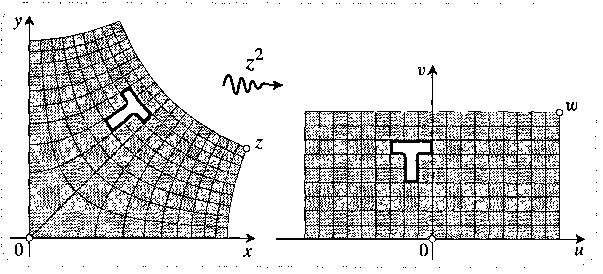
\includegraphics[height=3.0cm]{2021-1-C3/20210825_needham_fig2.pdf}$$

% (find-bortolossi7page (+ -238 256)    "matriz jacobiana")

% (find-books "__analysis/__analysis.el" "needham")
% (find-needhampage (+ 21 189) "Differentiation: The Amplitwist")
% (find-needhamtext (+ 21 189) "Differentiation: The Amplitwist")

% (find-fline "~/2021.1-C3/" "20210825_needham_fig1.jpg")


\newpage

% «exercicio-1»  (to ".exercicio-1")
% (c3m211jp 6 "exercicio-1")
% (c3m211ja   "exercicio-1")

{\bf Exercício 1.}

Desenhe um plano pros valores de $z$, à esquerda, e um plano pros
valores de $w=z^2$ à direita, como nas figuras do Needham. Desenhe no
planos dos `$z$'s os 9 valores de $z$ que têm $x∈\{0,1,2\}$ e
$y∈\{0,1,2\}$. Pra cada um desses 9 `$z$s calcule o `$w$
correspondente e desenhe ele no plano dos `$w$'s.


\newpage

% «preparacao-mini-teste»  (to ".preparacao-mini-teste")
% (c3m211jp 7 "preparacao-mini-teste")
% (c3m211ja   "preparacao-mini-teste")

\thispagestyle{empty}

\begin{center}

\vspace*{1.5cm}

\begin{tabular}{c}
{\bf \Large Exercícios de} \\
{\bf \Large preparação pro} \\
{\bf \Large mini-teste} \\
\end{tabular}

\end{center}

\newpage

No exercício 1 você descobriu as imagens

pela função $z \mapsto w$ de 9 {\sl pontos}. Agora você

vai descobrir as imagens de 9 {\sl retângulos}.

\msk

Sejam $α$ e $β$ dois reais positivos bem pequenos.

Vamos fazer os desenhos todos à mão, então você

pode usar $α=β=0.2$, ou $α=β=0.1$, algo assim ---

basta que $α^2$ e $β^2$ sejam ``desprezíveis'' no sentido

do Silvanus Thompson (e dos vídeos).

\msk

Em cada um dos 9 pontos você vai imaginar

um retangulinho de lados $α$ e $iβ$ ``apoiado nele'',

como o da figura do próximo slide...

\newpage

% (find-latexscan-links "C3" "20210827_rect_alpha_beta")
% (find-xpdf-page "~/LATEX/2021-1-C3/20210827_rect_alpha_beta.pdf")
$$\includegraphics[height=6.5cm]{2021-1-C3/20210827_rect_alpha_beta.pdf}$$

\newpage

...e você vai usar as derivadas pra encontrar uma

{\sl aproximação bastante razoável} pra imagem do

retangulinho apoiado em cada um dos 9 `$z_0$'s,

e vai desenhar essa aproximação apoiada no $w_0$

correspondente a aquele $z_0$.


\bsk
\bsk

O vídeo tem montes de explicações e dicas. Links:

\msk

{\scriptsize

\url{http://angg.twu.net/eev-videos/2021-1-C3-matriz-jacobiana-2.mp4}

\url{https://www.youtube.com/watch?v=D_YKka3RG9E}

}


\newpage

% «mt-dica-contas»  (to ".mt-dica-contas")
% (c3m211jp 11 "mt-dica-contas")
% (c3m211ja    "mt-dica-contas")

Se $γ=α+iβ$, então...

(Veja o vídeo!!!)
%
$$\scalebox{0.9}{$
  \begin{array}{rcl}
  w(z_0 + γ)  &=& w(z_0 + (α+iβ)) \\
              &=& w((x_0 + iy_0) + (α+iβ)) \\
              &=& w((x_0 + α) + i(y_0 + β)) \\
              &=& w(x_0 + α, y_0 + β) \\
              &=& w(x_0 + α, y_0 + β) \\
              &=& a(x_0 + α, y_0 + β) + ib(x_0 + α, y_0 + β) \\
              &=& (a(x_0 + α, y_0 + β), b(x_0 + α, y_0 + β)) \\
              &≈& (a + a_x α + a_y β, b + b_x α + b_y β) \\
              &=& (a,b) + (a_x α + a_y β, b_x α + b_y β) \\
              &=& (a,b) + \pmat{a_x & a_y \\ b_x & b_y} \pmat{α \\ β} \\
  w(z_0 + γ) - w_0 &=& \pmat{a_x & a_y \\ b_x & b_y} \pmat{α \\ β} \\
  \end{array}
  $}
$$


\newpage

{\bf Exercício 2.}

Qual é a imagem pela função $z \mapsto z^2$ da figura abaixo?

Note que o tamanho dos retangulinhos vai depender

dos valores de $α$ e $β$ que você escolheu...

% (find-latexscan-links "C3" "20210827_9_retangulinhos")
% (find-xpdf-page "~/LATEX/2021-1-C3/20210827_9_retangulinhos.pdf")
$$\includegraphics[height=5cm]{2021-1-C3/20210827_9_retangulinhos.pdf}$$




%\printbibliography

\GenericWarning{Success:}{Success!!!}  % Used by `M-x cv'

\end{document}

%  ____  _             _         
% |  _ \(_)_   ___   _(_)_______ 
% | | | | \ \ / / | | | |_  / _ \
% | |_| | |\ V /| |_| | |/ /  __/
% |____// | \_/  \__,_|_/___\___|
%     |__/                       
%
% «djvuize»  (to ".djvuize")
% (find-LATEXgrep "grep --color -nH --null -e djvuize 2020-1*.tex")

 (eepitch-shell)
 (eepitch-kill)
 (eepitch-shell)
# (find-fline "~/2021.1-C3/")
# (find-fline "~/LATEX/2021-1-C3/")
# (find-fline "~/bin/djvuize")

cd /tmp/
for i in *.jpg; do echo f $(basename $i .jpg); done

f () { rm -v $1.pdf;  textcleaner -f 50 -o  5 $1.jpg $1.png; djvuize $1.pdf; xpdf $1.pdf }
f () { rm -v $1.pdf;  textcleaner -f 50 -o 10 $1.jpg $1.png; djvuize $1.pdf; xpdf $1.pdf }
f () { rm -v $1.pdf;  textcleaner -f 50 -o 20 $1.jpg $1.png; djvuize $1.pdf; xpdf $1.pdf }

f () { rm -fv $1.png $1.pdf; djvuize $1.pdf; xpdf $1.pdf }
f () { rm -fv $1.png $1.pdf; djvuize WHITEBOARDOPTS="-m 1.0 -f 15" $1.pdf; xpdf $1.pdf }
f () { rm -fv $1.png $1.pdf; djvuize WHITEBOARDOPTS="-m 1.0 -f 30" $1.pdf; xpdf $1.pdf }
f () { rm -fv $1.png $1.pdf; djvuize WHITEBOARDOPTS="-m 1.0 -f 45" $1.pdf; xpdf $1.pdf }
f () { rm -fv $1.png $1.pdf; djvuize WHITEBOARDOPTS="-m 0.5" $1.pdf; xpdf $1.pdf }
f () { rm -fv $1.png $1.pdf; djvuize WHITEBOARDOPTS="-m 0.25" $1.pdf; xpdf $1.pdf }
f () { cp -fv $1.png $1.pdf       ~/2021.1-C3/
       cp -fv        $1.pdf ~/LATEX/2021-1-C3/
       cat <<%%%
% (find-latexscan-links "C3" "$1")
%%%
}

f 20210827_9_retangulinhos

f 20210827_rect_alpha_beta

f 20210825_needham_fig1
f 20210825_needham_fig2

f 20201213_area_em_funcao_de_theta
f 20201213_area_em_funcao_de_x
f 20201213_area_fatias_pizza



%  __  __       _        
% |  \/  | __ _| | _____ 
% | |\/| |/ _` | |/ / _ \
% | |  | | (_| |   <  __/
% |_|  |_|\__,_|_|\_\___|
%                        
% <make>

 (eepitch-shell)
 (eepitch-kill)
 (eepitch-shell)
# (find-LATEXfile "2019planar-has-1.mk")
make -f 2019.mk STEM=2021-1-C3-matriz-jacobiana veryclean
make -f 2019.mk STEM=2021-1-C3-matriz-jacobiana pdf

% Local Variables:
% coding: utf-8-unix
% ee-tla: "c3j"
% ee-tla: "c3m211j"
% End:
